\documentclass[12pt]{article}
\pagenumbering{arabic}
\pdfpagewidth 8.5in
\pdfpageheight 11in
\setlength\topmargin{0in}
\setlength\headheight{0in}
\setlength\headsep{0in}
\setlength\textheight{9.0in}
\setlength\textwidth{6.5in}
\setlength\oddsidemargin{0in}
\setlength\evensidemargin{0in}
\setlength\parindent{0.25in}
\setlength\parskip{0.25in}
\parskip 0.0pt
\usepackage[utf8]{inputenc}
\usepackage[english]{babel}
\usepackage{amsmath}
\usepackage{amsfonts}
\usepackage{amssymb}
\usepackage{amsbsy}
\usepackage{setspace}
\usepackage{graphicx}
\usepackage{tabularx,ragged2e,booktabs,caption}
\usepackage{float}
\usepackage{dcolumn}
\usepackage{natbib}
\usepackage{subfigure}

\begin{document}  


\begin{titlepage}
	\begin{center}

\vspace*{10 em}
\toprule[1.0pt]\\[0.2cm]
{ \huge \bfseries A Dynamic Model of Political Stability and Dissent \\[0.2cm] }
\bottomrule[1.0pt]

\large
\\[1.2cm]
\emph{Authors:}\\
Ethan \textsc{Spangler}, Washington State University\\
Ben \textsc{Smith}, University of Nebraska-Omaha 



\vfill

% Bottom of the page
{\large \today}
\end{center}



\begin{abstract}
The importance of political stability is well established and can affect all aspects of an economy. However, despite its significance, theoretical models of political stability remain underdeveloped. As demonstrated by the recent uprisings in the Middle East and populist fervor in the US and Europe; current models inadequately explain either. Our model extends the work of previous scholars by focusing on the interactions of a non-altruistic government and its citizenry. The government maximizes its own stability by choosing its level of public and security spending, subject to a resource constraint and the level of discontent from the citizenry. In turn, each member of the public chooses their level of dissent, based on their own preferences and the risk of punishment. Through simulation we determine the maximum exogenous shock that does not result in a revolution. The end result is a framework which can be used to develop a new index of political stability.
\end{abstract}

\end{titlepage}

\begin{spacing}{1.5}


\section{Intro}

The past decade has seen dramatic political shifts in both the developing and developed worlds. In December 2010 mass protests and demonstrations erupted across Tunisia, demanding an end to the autocratic regime of Ben-Ali. For years Tunisia had been plagued by corruption, high unemployment, inflation, and many other systemic problems that the government continuously failed to address. The Tunisian protests quickly turned into a full scale revolution as Ben-Ali was forced to flee the country a mere two months after protests began. Spurred by the success in Tunisia and facing the same governmental failures, long suppressed public outrage unleashed itself and cascaded through the rest of North Africa and the Middle East, resulting in what is now referred to as the Arab Spring. While the events of the Arab Spring are still unfolding, thus far it has resulted in complete regime changes in Tunisia, Libya, and Egypt; an on going civil war in Syria; and substantial political concessions in many other countries.  

While less explosive, the developed world has seen it's own manifestations of political instability. In the UK a referendum rejected continued membership in the EU, a move that surprised much of the world. In the US, Donald Trump, a man that has never held public office, rode a wave of populist rhetoric into the White House; beating a candidate considered to be a political insider. Other Western countries have seen formerly fringe parties either be elected into office or make substantial parliamentary gains. In each case, the policies and politicians were carried in to office by a public that felt that the previous governments had failed to address their concerns adequately.

Surface analysis of the Arab Spring and recent Western populism may find few parallels between them, but the two are more similar than many would like to admit. In both cases, the governments have each had continuously failed to address the concerns of the public. The only difference between the two is that with the Arab Spring, there were no nonviolent means to enact change to the government whereas in the West there are non-violent means to change the government, ie voting. So while the means may have differed, riots vs. ballots, the ultimate effect was the same, a change in government.  

Part of why these event were so surprising for so many, is the lack of a model concerning the interactions of a government and its citizens. A common view in economics is to view the government as that of a benevolent social planner, a fictitious  but theoretically convenient entity seeking to maximize welfare. Some theoretical developments have stepped away from absolute benevolence and introduce a measure of corruption (Acemoglu and Robinson 2001), but the overall set up remains largely unchanged. This paper steps away from the social planner model and seeks to construct a model of governance more nuanced than the social planner and robust enough to account for both authoritarian and democratic countries.  
  

%The importance of political stability is well established and can affect all aspects of an economy. However, despite its significance, measurement of political stability has remained underdeveloped. As demonstrated by the recent uprisings in the Middle East, Thailand, and Ukraine; large scale political changes are difficult to predict. The three commonly used measures of political stability are Political Risk Services (PRS), the Business Environment Risk Intelligence Index (BERI), and the Economist Intelligence Unit (EIU). Each of these indexes combine political, financial, and economic factors to assess a nation's political stability (Howell, 1998). The financial and economic portions are predominately based on quantitative data (foreign debt, inflation, GDP per capita, etc) while political factors are far more subjective. 

%Political factors are determined and scored by panels of experts (Howell, 1998). These experts are usually former diplomats and scholars. While these teams of experts can be quite large and knowledgeable, it is still a relatively small group of people trying to assess an entire nation and without a theoretical basis for their decisions. Since each index has political factors compose 33-66\% of their measure (Howell, 1998), if these experts are misinformed the validity of the index could be greatly affected which in turn would affect all research based on these indexes. Given in a twenty year study Tetlock (2005) was able to show that political forecasts based on expert opinion were only marginally better than random chance. It becomes quite apparent that a new method of assessing political stability is needed. Thus it is the goal of this paper to establish the theoretical basis for a new index of political stability; an index that factors in the dynamic relationship between those that rule and those that are ruled.  

%To highlight the issue of why a more robust measure of political stability is needed let us examine some examples and their related political stability analysis. The October 2005 PRS report on Thailand said ``unrest is not expected to threaten general stability, nor intensify to the point of endangering the [Thai Rak Thai Party's (TRT)] dominant political position...the chances of the TRT being forced from power at any point during the five year forecast period are slim..." Less than a year later a military coup ousted the Prime Minister Shinawatra and outlawed his TRT party, and began a period of political strife that continues to plague Thailand. The PRS report on Ukraine, published October 2012, stated that ``a repeat of the Orange Revolution...is unlikely." and ``Ukrainians are disillusioned but in general they possess little appetite for protest." Mass protests began in November 2013 and by February 2014 the Yanukovych regime had fallen. The PRS report on Tunisia, published October 2010, called Tunisia an ``oasis of stability" and postulated a 85\% probability that Tunisian dictator Ben Ali would retain power for the next 18 months. By January 2011, mass protests and revolt resulted in the dissolution of the ruling RCD party, the exile of Ben Ali to Saudi Arabia, and the establishment of an interim government. While it may be easy to critique these forecasts with the benefit of hindsight, these examples highlight the difficulty in predicting something as opaque and complex as political stability.\footnote{It should be noted that PRS publishes monthly reports on its surveyed countries but those are only available to its subscribers.} A new method of analyzing political stability is needed and we begin by developing a new theoretical framework. 

%I need to go back and properly cite these quotations
%I should also mention that PRS publishes monthly reports, but only those are only available to its subscribers. 

The structure of this paper is as follows: a review of the literature concerning political stability, our theory on the structure of political stability, simulations and analysis, and finally conclusion. Our goal in this paper is to form a coherent and testable model of political stability.   

\section{Related Literature}

The bulk of the literature concerning political stability focuses on the factors motivating revolt and revolution. Grossman (1991), Acemoglu and Robinson (2001), and MacCulloch (2001 and 2005) explore the role of income inequality in fomenting revolution. Other approaches concentrate on the role regime type plays (Guttman, 2014) or government institutions (Goldstone et al 2010; Acemoglu et al., 2012; Fukuyama, 2014). The general findings of these papers is that the more unequal a society is and the less effective its institutions, the more unstable the country will be. 

Diverging from the top down macroeconomic approach, other literature from the Public Choice field concerns the individual level. Tullock's (1971 and 1974) seminal works concerning the economics of rebellion focus on the paradoxical observation that while it seems inherently irrational for an individual to join a rebellion, objective evidence is to the contrary since revolutions have occurred and will continue to. In essence the problem is how do people cooperate enough to form a functional rebellion. Tullock answers this problem by focusing on the potential material gains that could come from a successful rebellion. Kurrild-Klitgaard (1997), Apolte (2010), and Bueno de Mesquita (2010) all build off of the foundation established by Tullock and offer their own solutions to the so called 'Paradox of Rebellion' but still remain within the game theoretic structure established by Tullock. 

It is felt by the authors of this paper that the focus on revolution, though valuable, does not capture the entirety of the situation. Revolution is the end point on a long process. A nation can exist for a long time in a state of low political stability but not descend into revolt; i.e. be stable in its instability. Thus, in a departure from the literature, we will be focusing on the decisions and dynamics that precipitate a revolution. By focusing on the dynamics preceding a revolution, we avoid the theoretical difficulties that have hampered the collective action problem explored by the literature on the paradox of rebellion.  

%umm, what do we call our approach? 

%Hmm, maybe I should look at this guy Theodore Gurr theorized in his 1970 book Why Men Rebel

"In perpetrating a revolution, there are two requirements: someone or something to revolt against and someone to actually show up and do the revolting." (Allen, 1975. pg 107). In this paper we adopt a similar mentality as Allen by incorporating the actions of both the government and the people. Our model extends the approach initiated by Acemoglu and Robinson (2001) and focuses on the dynamic interactions of a non-altruistic government and its citizenry. This paper bridges the institutional and public choice approaches to include both the effectiveness of government institutions and an individuals choice to dissent. The goal of this paper is not to predict the spark that ignites a revolution, but instead to measure the environment that allows a spark to turn into a revolution. Through simulation we explore how different countries with differing parameter values react and handle various exogenous shocks. The end result is a framework which can be used to develop a new index of political stability. Whereas current measures have no clear interpretation, ours would have the defined statistical interpretation of a probability a given event occurring. This makes it a far more robust and useful measure.

%Through simulation we determine the maximum exogenous shock that does not result in a revolution. This translates to a probability of failure of the state. The end result is a framework which can be used to develop a new index of political stability. Whereas current measures have no clear interpretation, ours would have the defined statistical interpretation of a probability a given event occurring. This makes it a far more robust and useful measure.    

\section{Theoretical Model}

The model begins in period 0. The catalyst the model is the initial amount total dissent, $D_0$. This $D_0$ can be thought of as either anarchists or remnants of the previous regime, their origin doesn't really matter just that it exists. A government then forms to manage and organize affairs, setting initial policy choices. The government maximizes political stability by choosing its level of public and security spending, subject to a resource constraint and the level of discontent from the citizenry. In turn, each member of the public chooses their level of dissent based on their own preferences and the probability of punishment. This dynamic repeats until state failure, which we will explicitly define later. 
 
\subsection{Individual's Problem}
Initial framing of the individual begins in the general sense as a household problem, 

\begin{equation}
	U(c,l) \text{ s.t. } M
\end{equation}

\noindent where utility, $U(c,l)$, is a function of consumption and leisure subject to an income constraint, $M$. The individual finds a solution for themselves. This represents the aspects of an individual's life that they have control over. However, the world being the imperfect place that it is, there are some things that an individual cannot control.  

The story is that in their daily lives, individuals face societal problems. It could be as mundane as a long line at the DMV. Perhaps they encountered a corrupt police officer. Another scenario could potential involve members of a different group harassing the individual. Maybe they saw a story about a wealthy, well-connected elite dodging criminal charges. Whatever the particular issue, it is a problem that the individual cannot directly solve themselves but it has negatively affected their life. These are societal issues that only a government could properly address. However, for whatever reason the government is unable and/or unwilling to address these problems completely to the satisfaction of the individual. Our origin for dissent is very similar to Gurr's (2015) concept of 'relative deprivation' wherein the perceived difference between a person's value exception and their value capabilities insights political violence. However, here we are emphasizing the relationship between the individual and their government. The incongruousness between an individual's expectations of what a government should do and the reality of what a government does do is the origin of dissent. So without any direct power to alter their situation the individual does what people usually do in such situations, they dissent. 

The individual uses a portion of what would be their leisure and instead uses it to dissent, which provides a cathartic release. Dissenting gives the individual some level of utility, with how much extra utility dictated by individual preferences and external parameters. Tullock (1971 and 1974) had a similar notion that there were potential non-material benefits of rebellion to the individual, but Tullock viewed it more as entertainment whereas we view dissent as therapeutic. Since the individual is only optimizing across a single variable, we can use a simple functional form wherein the individual maximizes utility from dissenting based on costs and benefits. 

\vspace{.5 em}
\noindent Individual's Problem:
\begin{equation}
{\underset{d_{i,t}}{\text{max }}}  U_{i,t}= \frac{{d_{i,t}}^{{x}_i}}{g_t * E} - P \left( \bar{d}_{t-1} \Bigg|\frac{D_{t-1}}{S_t},\sigma \right)d_{i,t}^A
\end{equation}

$ d_{i,t} $ is the amount individual $i$ dissents in period $t$ and is treated as a level variable wherein each period an individual chooses their level of dissent based on the situation they find themselves in and their own preferences. We assume that dissent takes only non-negative values, $d_{i,t}\geq0$. Different levels of $d_{i,t}$ have different interpretations. An individual with $d_{i,t}=0$ is interpreted as not dissenting, this person is either content with the government or too scared to dissent. Alternatively a positive value of $d_{i,t}$ can be interpreted as being more active. On the low end, $d_{i,t}>0$, could be contacting government representatives, attending open forums, voting for opposition parties, or kvetching about politics with colleagues. At the extreme end, $d_{i,t}>>0$, dissent takes on a more revolutionary bent: protests, riots, molotovs. Since individuals dissent during time they would otherwise be using for leisure there is a maximum amount a single individual can dissent for a given period, ${d_{i,t}}^{max}$. 

$x_i$ is the exponent that represents an individual's level of activism with respect to dissenting. We assume $x_i \sim logN(0,1)$, the Log-Normal PDF. Different values of $x_i$ have different interpretations. As show in Figure 1, an individual with a $x_i$ on the left of the distribution (the darker shades) could be seen an individual with high anxiety when it comes to dissenting. However, as we move to the right of the distribution (lighter shades), the individual become more amenable to dissent. Near the peak, these individuals might be comfortable discussing their frustrations among close peers (``Dinner Party Dissenters") but more active actions is unlikely. As we move to the far right, each higher value of $x_i$ represents a more activist role the individual would be willing to undertake. Since we have made an assumption on the distribution of activism, this allows us to determine how much dissent there will be in a country each period for given government policy choices.    

\begin{figure}[htb]
\centering 
\caption{Activism Plot, $x_i \sim logN(0,1)$}
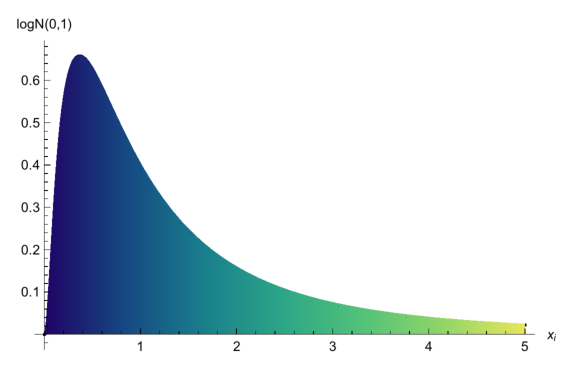
\includegraphics
[width=0.45\textwidth]{Activism_Plot.eps} 
\end{figure}

$E$ and $g_t$ reduce the amount of utility an individual gets from dissenting. $E$ is an exogenous parameter assessing and individual's environment each period. By environment we mean an individual's living situation within a country: unemployment, healthcare, safety, equality, etc. $E$ allows us to weigh the validity of dissent for comparisons across countries. Dissent in a country where conditions are good (``first world problems") are far less meaningful than in countries with more difficult situations. By weighing dissent based on the circumstances of a country, we are better able to establish a framework of political stability that works for both developed and developing countries. $g_t$ is per capita government spending($g_t=\frac{G_t}{N_t}$ where $N_t$ is the population) and is treated as given in the individual's problem. $g_t$ represents how much the government services are given to each citizen. Since this is a pure public good, the government cannot restrict who receives this, thus the individual receives this benefit regardless of their level of dissent. 

$ P \left( \bar{d}_{t-1} \Bigg|\frac{D_{t-1}}{S_t},\sigma \right)$ is a the probability of being caught dissenting against the government and it follows the Log-Normal PDF. $S_t$ is government resources spent on quelling dissent and is treated as given in the individual's problem. $D_{t-1}$ is the preexisting total dissent. $\bar{d}_{t-1}$ is the average individual dissent from the previous period. $\sigma$ represents policing effectiveness. For low $\sigma$ the police are extremely prompt at arresting those that dissent beyond acceptable limits. For higher $\sigma$ the probability of being arrested becomes more spread out. For practical empirical purposes $\sigma$ is the ratio of $\frac{\text{Total Reported Crime}}{\text{Crimes Cleared}}$. While not perfect, it does provide some insight into police effectiveness. $A$ this is the punishment parameter for dissenting and is structured such that $A>1$. Since the punishment should fit the crime, an individual is punished based on their level of dissent. 

An assumption with $P \left( \bar{d}_{t-1} \Bigg|\frac{D_{t-1}}{S_t},\sigma \right)$ is that the amount an individual dissents does not affect their probability of being caught for dissenting. The reasoning is that the amount of dissent a single individual could produce is insignificant within an entire nation ($d<<D$), a drop in the ocean so to speak. That said, if an individual is caught they will be punished based on the amount they have dissented. The benefit of structuring $P$ in this way, is that even though it is exogenous to an individual, it is still endogenous to the system. This will allow the probability of being caught alter as conditions change.   



%While previous works used various measures to assess government institutional quality, many of those measures have the same subjectivity problem as the political stability measures discussed previously. 


%By focusing on dissent and weighting it by objective, quantitative data ($g$ and $E$) we can actually get a more accurate view of institutional quality by looking at how frustrated people are with these institutions.     

\subsection{Government's Problem} 

In our view there is no reason to think a government exclusively seeks to maximizes social welfare. Evidence abounds with leaders less than sympathetic towards the plights of their constituents: North Korea, Syria, the US Congress. It would then seem that the primary goal of leaders is retaining power, obtaining some hidden benefit that is contingent upon sustained stability. Thus it becomes the goal of government to maximize political stability. 

The Government's problems begins with the with the Leader's problem. As stated previously stated, leaders receive some benefit from holding power. The leaders could be taking funds from the treasury, receiving a portion of resource export profits, or have firms they're heavily invested in receive lots of lucrative no-bid government contracts. Whatever the case, the leaders gets this benefit (and the utils) only if they are in power. So leaders seeks to maximize their own utility subject to political stability ($\Lambda_t$) remaining positive.

\vspace{.5 em}
\noindent Leaders' Problem:
\begin{equation}
	 \text{max } U_t(B_t) \begin{cases}
		>0 \text{ if } \Lambda_t > 0 \\
		= 0 \text{ otherwise} 	
	\end{cases}
\end{equation} 

\noindent where $B_t$ is the benefit from holding power that the leader takes. However, this benefit is not costless and it diminishes the resources the government has to use to maintain stability: 

\vspace{.5 em}
\begin{equation}
	R_t={\Pi}_t-B_t
\end{equation} 

\noindent where ${\Pi}_t$ is the total amount of resources taken in by the state, before the leader takes their cut. This leaves $R_t$, the remaining resources that the government has to use to maintain stability. The leader can line their pockets but must be careful not to take too much or they'll facilitate their own demise. With the leader's problem established, we move on to the task of maintaining stability.   
\vspace{.5 em}

\noindent Government's Problem:
\begin{equation}
{\underset{G_t,S_t}{\text{max }}} \sum\limits_{t=1}^{T^*} \beta^t {\Lambda}_t = \sum\limits_{t=1}^{T^*} \beta^t\left(\frac{G_t}{D_{t-1}}-\Phi\right)^\alpha \left(\frac{S_t}{D_{t-1}}-\Omega\right)^\gamma   \text{s.t. } G_t+S_t=R_t
\end{equation}

It is the goal of the government to maximize stability over time. The stability function uses a Stone-Geary functional form. $G_t$ is government spending on government services. Basically $G_t$ provides all the things we expect a functioning government to provide (schools, hospitals, DMVs, etc). $S_t$ is security spending, resources used to suppress the population. If $G_t$ is the carrot, $S_t$ is the stick. These are resources that the government uses to suppress the public and maintain order. 

%Why did we use a Stone-Geary functional form? 

$\Phi$ and $\Omega$, are the anarchy conditions, representing the minimum amount of government and security spending needed in order for the government to function at even a basic level. If either of these minimum conditions are not met for whatever reason, such as an exogenous shock, stability goes to zero and you have a revolution. This is why the problem is maximized to $T^*$ not $\infty$, since all governments eventually fail. Should $\Lambda_t \leq 0$, that would signify the state has broken down and a revolution has taken place, resetting the system. $\beta^t$ is the government's discount factor for stability. 

$\alpha$ and $\gamma $ are parameters representing how much a government favors using $G_t$ and $S_t$ respectively. It is assumed that $\alpha+\gamma=1$. One would expect a democracy to favor $G$ over $S$ ($\alpha > \gamma$) but the opposite would hold for a totalitarian regime ($\alpha < \gamma $). No country can forgo either completely; even the most kleptocratic and despotic regimes provide some form of service to citizens and the most utopian societies still have a police force. $G_t+S_t=R_t$ is the government resource constraint. No government can spend unlimited amounts of resources, so they face a constraint. $R_t$ is government resources available to the decision makers each period. 

$D_{t-1}$ is total dissent from the previous period. Dissent reduces the effectiveness of government policy and in turn makes it difficult for the government is retain power. Ruling those that do not wish to be controlled will always be more difficult. Consider the difficulty of herding cats as opposed to sheep, the same applies to an unhappy public. Thus, the more dissent that exists in the system, the more difficult it will be for the government to maintain stability.  

As shown, the government reacts to the previous period of dissent whereas the individual reacts to the current period. The result is that the government cannot keep up with the situation on the ground. This bureaucratic delay is the source of instability. When $D_t \approx D_{t-1}$ the instability is small and manageable, but when $D_t \not\approx D_{t-1}$ the state may misallocate resources and the possibility of state failure increases. Continued incongruences could result in the situation spiraling out of control. 

\section{Solving the Model}

This is a two stage dynamic interaction between the government and the public. In the initial period the government sets initial policy $G_1$ and $S_1$ based on some starting value of $D_0$, the initial total dissent. $D_0$ can be interpreted a handful of ways: they could be from a group of anarchists (they hate all government) or maybe the losers in the contest that established the current government. Whatever their origins we just need an initial level of dissent to be greater than 0. Since no government has ever formed without some form of acrimony, this is not an unreasonable assumption. We can solve for an equilibrium through backwards induction, the goal being to determine dynamics of $D_t$. So we'll start with the individuals problem. 

\subsection{Individual's solution}

%It must be stated that there is no analytic solution to an individuals demand for dissent, which we will call $\overline{d}_{i,t}$. Demand for dissent must be numerically determined in simulations, which is discussed in the next section. 

The first step in determining individual demand for dissent is first discussing the scenarios which do and do not facilitate individual dissent. This requires examining the first order and second order conditions. 
 
\vspace{.5 em}
\noindent Differentiating the individual problem with respect to $d_{i,t}$ we obtain the FOC: 
\begin{equation}
\frac{dU}{dd_{i,t}} = x_i \frac{{d_{i,t}}^{x_i -1}}{E g_t} - P\left(\bar{d}_{t-1} \Big|\frac{D_{t-1}}{S_t},\sigma \right)Ad_{i,t}^{A-1}  
\end{equation}

\noindent Differentiating again with respect to $d_{i,t}$ we obtain the SOC: 

\begin{equation}
\frac{d^2U}{dd_{i,t}^2}=(x_i -1) x_i \frac{{d_{i,t}}^{x_i -1}}{E g_t} - P\left(\bar{d}_{t-1} \Big|\frac{D_{t-1}}{S_t},\sigma \right)(A-1)Ad_{i,t}^{A-2}  
\end{equation}

\noindent For the $\frac{dU}{dd_{i,t}}$ and $\frac{d^2U}{dd_{i,t}^2}$ Let:    
\begin{center}
$\underbrace{ x_i \frac{{d_{i,t}}^{x_i -1}}{E g_t}}_\textrm{H} - \underbrace{P\left(\bar{d}_{t-1} \Big|\frac{D_{t-1}}{S_t},\sigma \right)Ad_{i,t}^{A-1}}_\textrm{I}$  	
\end{center}

\noindent and: 

\begin{center}
$\underbrace{(x_i -1) x_i \frac{{d_{i,t}}^{x_i -2}}{E g_t}}}_\textrm{J} -\underbrace{P\left(\bar{d}_{t-1}\Big|\frac{D_{t-1}}{S_t},\sigma \right)(A-1)Ad_{i,t}^{A-2}}_\textrm{K}$  
\end{center}

\noindent Then the various scenarios are: 
\begin{enumerate}
\item If $x_i<0$, then $\frac{dU}{dd_{i,t}} < 0$ and $d_{i,t}=0$. 
\item If $x_i>0$ and $H<I$, then $\frac{dU}{dd_{i,t}} < 0$ and $d_{i,t}=0$. 
\item If $1>x_i>0$ and $H>I$; then utility is maximized when $\frac{dU}{dd_{i,t}}=0$, $\frac{d^2U}{dd_{i,t}^2}<0$, and $d_{i,t}>0$.  
\item If $x_i>1$, $H>I$, and $J<K$; then utility is maximized when $\frac{dU}{dd_{i,t}} = 0$, $\frac{d^2U}{dd_{i,t}^2}<0$, and $d_{i,t}>0$. 
\item If $x_i>1$, $H>I$, and $J>K$, then $\frac{dU}{dd_{i,t}} > 0$, $\frac{d^2U}{dd_{i,t}^2}>0$, and $d_{i,t}={d_{i,t}}^{max} $. 
\end{enumerate}

Scenarios 1 through 4 pose very little to be concerned about, providing a nice distribution of dissenters and non-dissenters amongst the populace. The $\text{5}^{\text{th}}$, however, requires a bit more explanation. Given the previously stated income constraint, $M$, and by extension the maximum possible amount of dissent, ${d_{i,t}}^{max}$; during situations in which $\frac{dU}{dd_{i,t}}$ and $\frac{d^2U}{dd_{i,t}^2}$ are positive the individual would merely dissent the maximum amount possible, ${d_{i,t}}^{max}$.  

With our various scenarios outlined we can now move on to the process of deriving individual demand for dissent, which is a simple algebraic process. 

\vspace{1 em}
\noindent Begin with the first order condition: 

\begin{equation}
	\begin{aligned}
\frac{dU}{dd_{i,t}}=& 0\\ 
x_i \frac{{d_{i,t}}^{x_i -1}}{g_t E} - PAd_{i,t}^{A-1}=& 0 \\
	x_i \frac{{d_{i,t}}^{x_i -1}}{g_t E} =& PAd_{i,t}^{A-1}\\
		d_{i,t}=& \left(\frac{g_tEPA}{x_i} \right)^{\frac{1}{x_i -A}}\\ 	
	\end{aligned}
\end{equation}

We shall call this solutions ${d_{i,t}}^*$ and use it to determine the expected total dissent, $D_t$. 

%To avoid this in simulation, if a random draw of $x_i$ is one such that it makes the $SOC>0$ it will be automatically lowered to the maximal value, $x_{max}$, where $SOC<0$ holds. This constrains should not prove too onerous.       
   
\subsection{Total Dissent}
 
To find the expected total dissent, we integrate $\{{d}_{i,t}}^*$ times the Log-Normal PDF, $f(x)$, across the relevant range of $x_i$, $0$ to $x_{max}$, will give the average amount of dissent per capita in a country. Multiplying this by the population, $N_t$, gives the expected total dissent, $D_t$.

\begin{equation}
	\begin{aligned}
D_t=& N_t \int_{0}^{x_{max}} {{d}_{i,t}}^* f(x) dx \\	
D_t	=& N_t \int_{0}^{x_{max}} {{d}_{i,t}}^* \frac{1}{x\sigma \sqrt{2\pi}}exp  \left( -\frac{(lnx-\mu)^2}{2\sigma^2} \right)  dx \\	
	\end{aligned}
\end{equation}

As you may be able to tell, a solution for total dissent cannot be analytically determined so we must rely on numerical simulation which will be discussed in the next section. This will be discussed further in the simulation section. 

\subsection{Government Solution}

To solve the government's problem we need a Lagrangian.
\begin{equation}
\mathcal{L} = \left(\frac{G_t}{ D_{t-1}}-\Phi\right)^\alpha \left(\frac{S_t}{ D_{t-1}}-\Omega\right)^\gamma  +\lambda[R_t-G_t-S_t] 
\end{equation}
Take the FOCs with respect to $G_t$ and $S_t$, then simplify:

\begin{equation}
    \begin{aligned}
        G_t\text{: } \alpha \left(\frac{G_t}{ D_{t-1}}-\Phi\right)^{\alpha-1} \frac{1}{ D_{t-1}} \left(\frac{S_t}{D_{t-1}}-\Omega\right)^\gamma  -\lambda &=0  \\
S_t\text{: } \gamma  \left(\frac{G_t}{ D_{t-1}}-\Phi\right)^{\alpha} \frac{1}{D_{t-1}} \left(\frac{S_t}{D_{t-1}}-\Omega\right)^{\gamma -1} -\lambda &=0 \\
\alpha \left(\frac{G_t}{D_{t-1}}-\Phi\right)^{\alpha-1} \frac{1}{ D_{t-1}} \left(\frac{S_t}{D_{t-1}}-\Omega\right)^\gamma  &= \gamma  \left(\frac{G_t}{ D_{t-1}}-\Phi\right)^{\alpha} \frac{1}{ D_{t-1}} \left(\frac{S_t}{ D_{t-1}}-\Omega\right)^{\gamma -1} \\
\alpha \left(\frac{S_t}{ D_{t-1}}-\Omega \right) &= \gamma  \left( \frac{G_t}{ D_{t-1}}-\Phi \right) \\
G_t&= D_{t-1}\left[\frac{\alpha}{\gamma } \left(\frac{S_t}{ D_{t-1}} -\Omega \right)+\Phi \right]
    \end{aligned}
\end{equation}

\noindent Plug this into the government resource constraint. 

\begin{equation}
    \begin{aligned}
        S_t+G_t&=R_t \\
        S_t+  D_{t-1}\left[\frac{\alpha}{\gamma } \left(\frac{S_t}{ D_{t-1}} -\Omega \right) +\Phi \right]  &= R \\
S_t+ \frac{\alpha S_t}{\gamma } -\frac{\alpha  D_{t-1} \Omega}{\gamma } +D_{t-1}\Phi &=R_t \\
S_t\left(1+\frac{\alpha}{\gamma }\right) &= R_t+ \frac{\alpha D_{t-1} \Omega}{\gamma } - D_{t-1}\Phi \\
S_t\left(\frac{\gamma  + \alpha}{\gamma }\right) &= R_t - D_{t-1} \left(\Phi - \frac{\alpha  \Omega}{\gamma } \right) 
    \end{aligned}
\end{equation}

\noindent Solve for $S_t$ and we get
\begin{equation}
S_t=\frac{\gamma }{\gamma  +\alpha} \left[ R_t - D_{t-1} \left(\Phi - \frac{\alpha}{\gamma }\Omega \right) \right]
\end{equation}
\noindent This is the government's security equation. We repeat the same steps to find $G_t$. 
\begin{equation}
G_t=\frac{\alpha}{\gamma  +\alpha} \left[ R_t - D_{t-1} \left(\Omega - \frac{\gamma }{\alpha}\Phi \right) \right]
\end{equation}

%The solutions for the government problem are combined with the results from the individuals problem to form the basis of our simulations. 

\section{Simulation} 

Given that a complete analytic solution for the theoretical model is not possible, numerical methods of simulation must be employed. To do this we developed eight country archetypes to test. While there are endless possible combination of the parameters, these 8 were chosen because they represent a broad range of characteristics and provide the most theoretical insight as to how differing parameter values affect stability. The values used in the simulations are based on extrapolations of real world data but are stylized to fit within the confines of the simulation. The explanation of each simulated country includes a list of which real world countries were used as a basis for forming the parameters values. 

\begin{table}[]
\centering
\begin{tiny}
\caption{Parameter Basis}
\begin{tabular}{llll}
\toprule
\textbf{Label} & \textbf{Variable} & \textbf{Basis} & \textbf{Source} \\ \hline
$\alpha$ & preference for G & specified &  \\
\textbf{$\gamma$} & preference for S & specified &  \\
\textbf{$R$} & Government resources & GDP & World Bank \\
$\Phi$ & S fixed costs & estimated & World Bank \\
\textbf{$\Omega$} & G fixed costs & estimated & World Bank \\
\textbf{$\sigma$} & Security effectiveness & $\frac{\text{Total Reported Crime}}{\text{Cleared Crimes}}$ & US FBI Crime Statistics \\
\textbf{$A$} & Dissent punishment & Political Freedom Score & Freedom House \\
\textbf{$E$} & Quality of life & Human Development Index & UN \\ \hline
\end{tabular}
\end{tiny}
\end{table}

Table 1 details the origin of the values used for the parameters in the simulations. Preference($\alpha$ and $\gamma$) values were specified by the authors to provide theoretical contrast between countries, but were influenced in part by estimates taken from the same analysis used for the anarchy conditions ($\Omega$ and $\Phi$) based on data from sample countries estimated from nonlinear least squares. Government resources, $R$, are based on GDP figures. $\sigma$ represents the effectiveness of security forces in suppressing dissent. 

The value of $\sigma$ was based on the ratio of total reported crime over total cleared\footnote{Cleared meaning that there was a resulting arrest. This was used over merely counting arrest because some criminals commit multiple crimes.} crime. In 2014 there were over 9.4 million violent (murder, assault, rape) and property (theft, larceny, vandalism) crimes in the US. Of these crimes, 2.2 million were cleared. The ratio of these provides an approximate $\sigma$ value of 4 which is what was used as a starting value in the simulations. Due to data limitations regarding crime rates around the world, this initial value of $\sigma$ was applied to the other simulation parameters with minor changes to create theoretical variation. 

$A$ is based on the Political Rights scores from Freedom House on a scale of 1\footnote{For computational reasons explained earlier a minimum value of 1.1 is used for simulation.} being the most free and 7 being the least. $E$ is based on the the UN's Human Development Index. Population is held constant between all simulated countries, with $N=10,000$. Since we are dealing with a smaller population than most countries, GDP values have been scaled accordingly, but the same relative GDP per captia remains. 

Simulations were conducted using Mathematica. For all simulations only 100 periods were analyzed. This was done because the authors are more concerned with the short-term fluctuations in stability than asymptotics. The following is a brief synopsis of each simulated country:  

%It must be emphasized that these simulations are meant to be stylized representations of various country archetypes that and no  

%based off of theoretical constructs (cite people)

%Consult the old Developement Lit: 
\begin{itemize}
	\item \textbf{Freedonia:} meant to represent the developed, socialist, and soft-power focused Western states. As such the parameters features a wealthy and efficient government, a preference for using government services to quell dissent, low punishment for those that are caught dissenting, and a high quality of life for citizens. Countries used for parameter basis: Canada, Japan, Western Europe, and Scandinavia. 
	\item \textbf{`Merika:} very similar to Freedonia in terms of preferences but slightly more disposed to using force to suppress dissent and slightly reduced quality of life. Countries used for parameter basis: Australia, South Korea, UK, and US. 
	\item \textbf{Kleptopia:} the antithesis of Freedonia. Kleptopia is a wealthy developed state but instead prefers brute force methods to maintain stability. Kleptopia also has a lower quality of life for its citizens. Country used for parameter basis: Russia.  
	\item \textbf{Cathay:} more balanced in preferences but with a slight list towards suppression. Is representative of states on the cusp of political and economic development. Punishment for dissenting is still quite high but quality of life is decent. Countries used for parameter basis: Brazil, China, India.   
	\item \textbf{Rentistan:} typical wealthy rentier state. Has equal preferences for both government services and suppression but also has low quality of life for it's citizens and is prone to corruption and inefficiency. Countries used for parameter estimates: Nigeria, Qatar.\footnote{There was insufficient data from other resource rich states, such as the Gulf States.} 
	\item \textbf{Develpolus:} the prototypical developing nation. Has equal preferences in regards to methods of maintaining order but is poor, has a low quality of life, and the government is either inefficient, corrupt, or both; leading to higher fixed costs. Countries used for parameter basis: Jordan, Kenya, Nepal.  	
	\item \textbf{Bellicostia:} similar to Kleptopia but lacks both the resources and skills. Resources are limited but are used primarily on suppression. Indicative of small autocratic states.  Countries used for parameter estimates: Iran, Pakistan, Syria. 
	\item \textbf{Hippieberg:} similar to Freedonia but lacks both the resources and skills. There is a preference for using government services over suppression but has few resources. Countries used for parameter basis: Bhutan, Uruguay, Baltic states.  
\end{itemize}

%Here is the table with the actual Parameter values. 

\begin{table}[]
\centering
\begin{tiny}
\caption{Parameter Values}
\begin{tabular}{lcccccccc}
\toprule
                    & \textbf{Freedonia} & \textbf{`Merika} & \textbf{Kleptopia} & \textbf{Cathay} & \textbf{Rentistan} & \textbf{Develpolus} & \textbf{Bellicostic} & \textbf{Hippieberg} \\ \hline
\boldmath{$\alpha$}   & 0.9              & 0.8              & 0.1                & 0.4             & 0.5                & 0.5                 & 0.1                  & 0.9                 \\
\boldmath{$\gamma$}   & 0.1                & 0.2              & 0.9                & 0.6             & 0.5                & 0.5                 & 0.9                  & 0.1                 \\
\textit{\textbf{R}} & 350,000,000        & 350,000,000      & 350,000,000        & 150,000,000     & 300,000,000        & 100,000,000         & 50,000,000           & 50,000,000          \\
\boldmath{$\Phi$}     & 17,500,000         & 17,500,000       & 52,500,000         & 1,500,000       & 105,000,000        & 35,000,000          & 500,000              & 14,500,000          \\
\boldmath{$\Omega$}   & 17,500,000         & 17,500,000       & 17,500,000         & 6,000,000       & 105,000,000        & 35,000.00           & 14,500,000           & 500,000             \\
\boldmath{$\sigma$}   & 3                  & 3                & 3                  & 6               & 9                  & 9                   & 5                    & 5                   \\
\textit{\textbf{A}} & 1.1                & 1.1              & 6                  & 6               & 5                  & 5                   & 6                    & 1.1                 \\
\textit{\textbf{E}} & 0.9                & 0.85             & 0.7                & 0.7             & 0.7                & 0.5                 & 0.6                  & 0.6                 \\
\textit{\textbf{N}} & 10,000             & 10,000           & 10,000             & 10,000          & 10,000             & 10,000              & 10,000               & 10,000 \\ \hline            
\end{tabular}
\end{tiny}
\end{table}

\subsection{Initial Dissent}

The first set of simulations focus on how states adapt to different levels of initial dissent, $D_0$. Many new countries face high levels of initial dissent, which often affects their stability. After WWII, decolonizations resulted in the creation of many new countries. However, many of the governments of these young countries fell shortly after because they could never overcome the initial enmity of their creation. 

The first simulation set contrasts when countries form under low and high initial dissent. Figure 2, depicts a near perfect scenario wherein there is almost no initial dissent ($D_0 = 1$) while Figure 3 shows our countries starting with a high level of initial dissent ($D_0 = 100$). It should be noted that while it may seem that these are flat lines, there is period to period variation.  

In both Figures 2 and 3 we see that countries that rely more heavily on suppression experienced substantial variation in their stability levels regardless of the resources available to the state. Cathay and Bellicostia saw their stability levels oscillate throughout the entire duration of the simulation without ever achieving a level of consistency on par with their neighbors. In striking contrast to the rest, Kleptopia immediately plunged into negative values. This is despite the fact that Kleptopia has considerably more resources than either Cathay or Bellicostia.  

%What should happen is that High Initial Dissent follows the same patterns as initial low, just at a lower level. This makes the countries more vulnerable to exogenous shocks that might arise. 


\begin{figure}[htb]
\centering 
\caption{Low Initial Dissent, $D_0=1$}
\subfigure{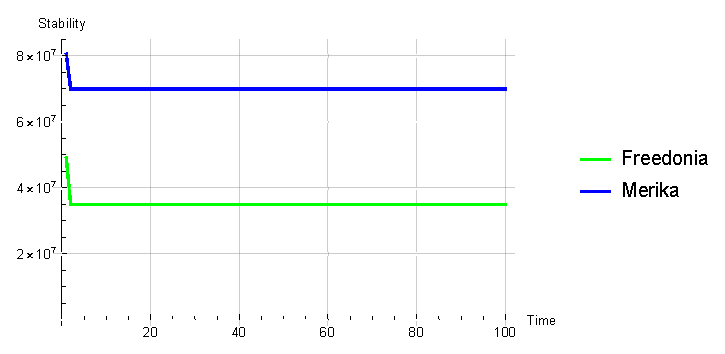
\includegraphics
[width=0.45\textwidth]{Low_Initial_Dissent_1.eps}} 
\subfigure{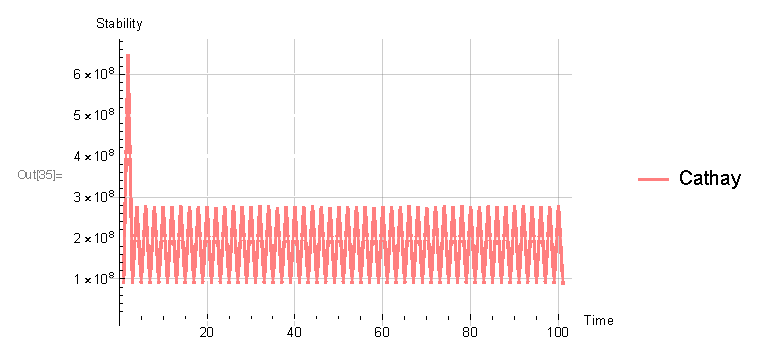
\includegraphics
[width=0.45\textwidth]{Low_Initial_Dissent_2.eps}} 
\subfigure{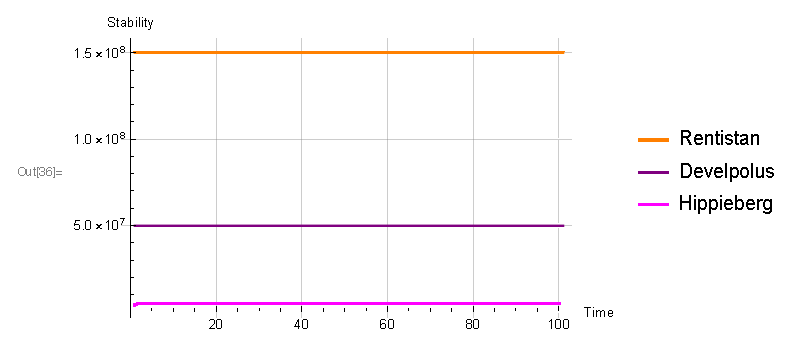
\includegraphics
[width=0.45\textwidth]{Low_Initial_Dissent_3.eps}} 
\subfigure{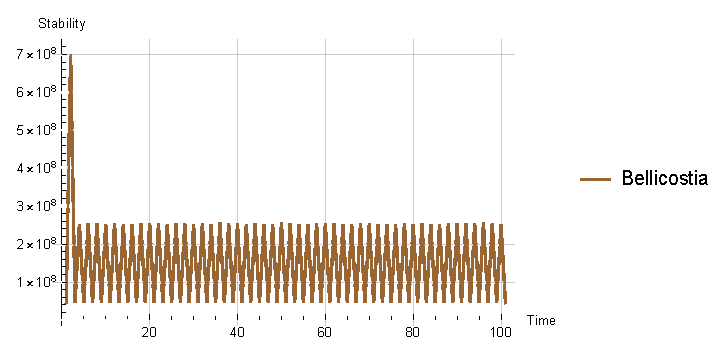
\includegraphics
[width=0.45\textwidth]{Low_Initial_Dissent_4.eps}} 
\subfigure{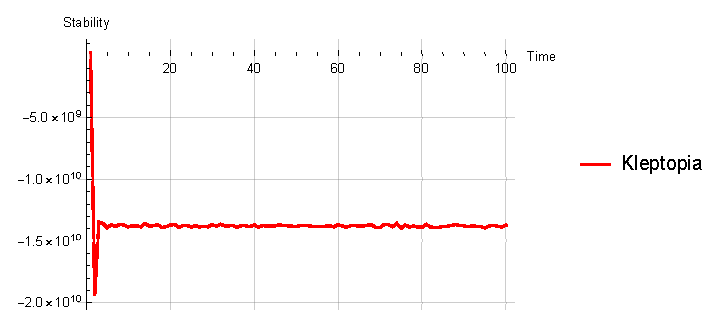
\includegraphics
[width=0.45\textwidth]{Low_Initial_Dissent_5.eps}} 
\end{figure}

Kleptopia's immediate plunge into instability, even under perfect circumstances, perhaps reflects the inherent unsustainability of such a preference and parameter set. Considering that Russia is the only current real world example that even comes close to approaching the extreme parameters of Kleptopia, reinforces this point. Overall, the plots adhere to our earlier point that countries can be stabile in their instability, exemplified especially by Cathay and Bellicostia, since every country that could achieve stability in the initial stage was able to perpetuate itself.   



%Kleptopia immediate plunged into negative values of stability, this aligning with Acemoglu's notion of autocractic nightmare   

In Figure 3, we see the stability plots of countries with a much high level of initial dissent, $D_0=100$. Generally, each country behaves very similarly as in Figure 2, but achieves a lower average stability level. This can be seen most prevalently with Freedonia, `Merkia, and Bellicostia. Freedonia and `Merika see substantial drops on their level of stability but remain consistent. Bellicostia no longer has the initial spike in stability, but instead goes right into its oscillating pattern.   

\begin{figure}[htb]
\centering 
\caption{High Initial Dissent, $D_0=100$}
\subfigure{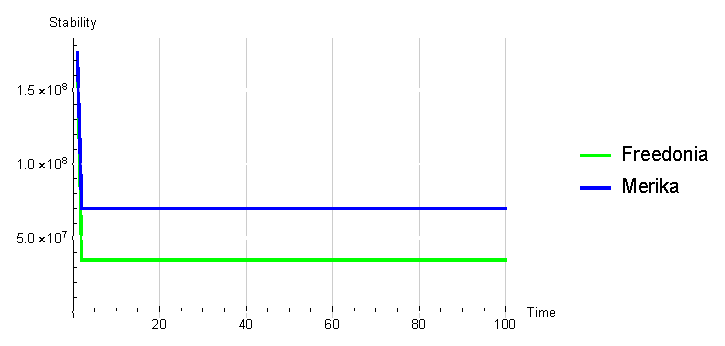
\includegraphics
[width=0.45\textwidth]{High_Initial_Dissent_1.eps}} 
\subfigure{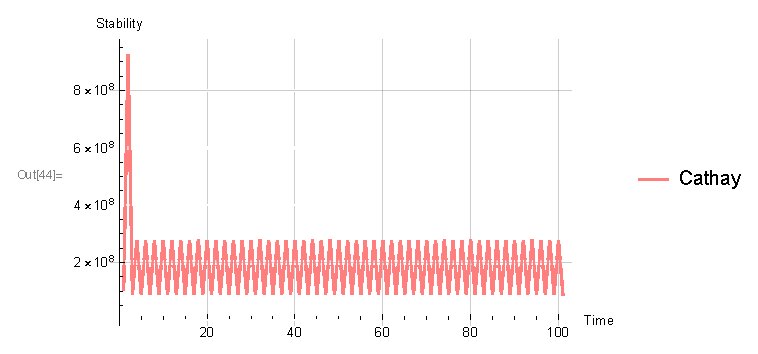
\includegraphics
[width=0.45\textwidth]{High_Initial_Dissent_2.eps}} 
\subfigure{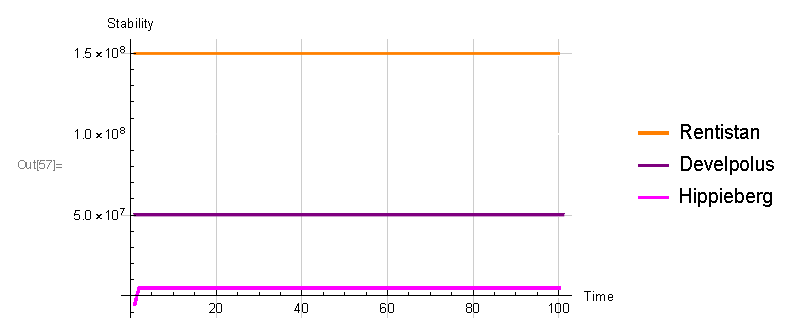
\includegraphics
[width=0.45\textwidth]{High_Initial_Dissent_3.eps}}
\subfigure{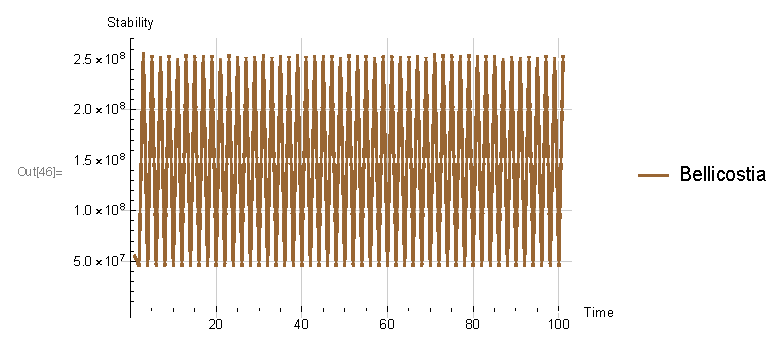
\includegraphics
[width=0.45\textwidth]{High_Initial_Dissent_4.eps}}
\subfigure{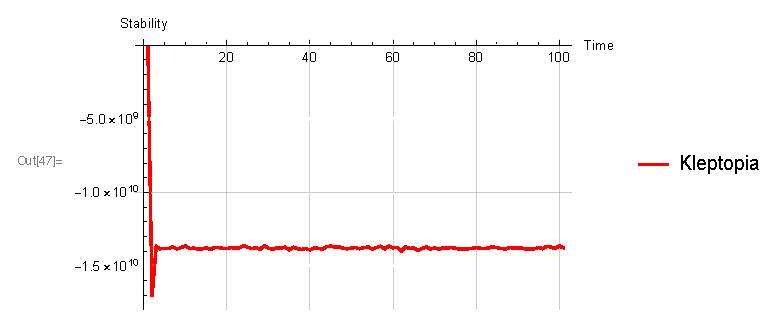
\includegraphics
[width=0.45\textwidth]{High_Initial_Dissent_5.eps}} 
\end{figure}


\subsection{Shocks}

Another interest was how robust various countries types are to various exogenous shocks. All shocks are simulated under the same conditions: the countries are simulated under conditions of low initial dissent ($D_0 = 1$), but then at period 50 a shock occurs in one of the parameters listed below and the effects of the shock are observed for the remainder of the run. The magnitude of the shocks are either a 25\% increase or decrease in the parameter, whichever would negatively affect the stability of a state.  

\begin{itemize}
	\item \boldmath{$R$:} the government resources are severely cut. Examples include the president emptying the treasury and fleeing to a non-extraditing country, currency devaluation, or massive recession/depression. Whatever the reason, the state now has less resources available to it.  
	\item \boldmath{$\Omega,\Phi$:} the government is hit with new levels of corruption/incompetence and more resources must be spent on the anarchy parameters. 
	\item \boldmath{$E$:} the quality of life suddenly drops. Mass joblessness, public health crisis, environmental degradation. 
	\item \boldmath{$\sigma$:} the government is less effective at catching people that dissent. Propagation of social media eases coordination of protesters, the police strike, pressure from human rights groups.     
\end{itemize}

\subsubsection{Resource Shocks} 

\begin{figure}[htb]
\centering 
\caption{Resource Shock}
\subfigure{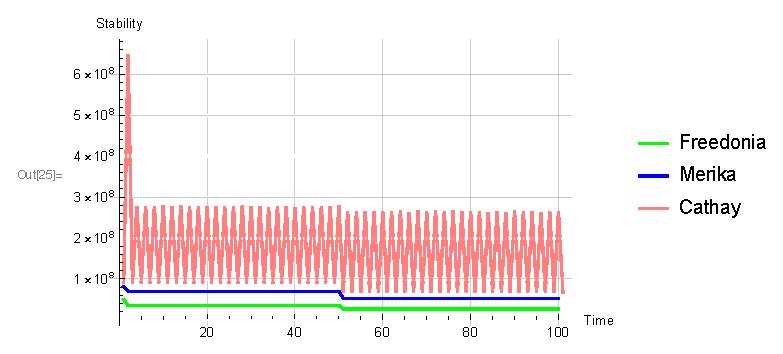
\includegraphics
[width=0.45\textwidth]{R_Shock_1.eps}} 
\subfigure{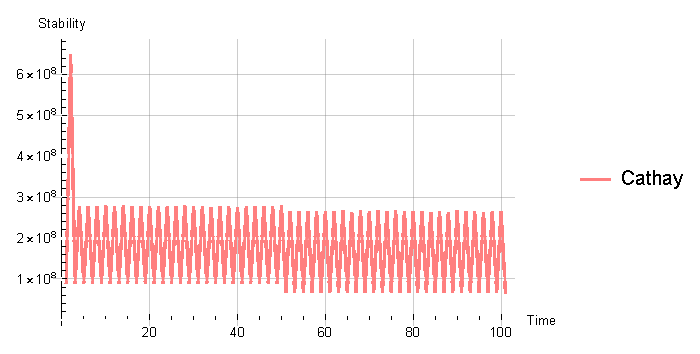
\includegraphics
[width=0.45\textwidth]{R_Shock_2.eps}} 
\subfigure{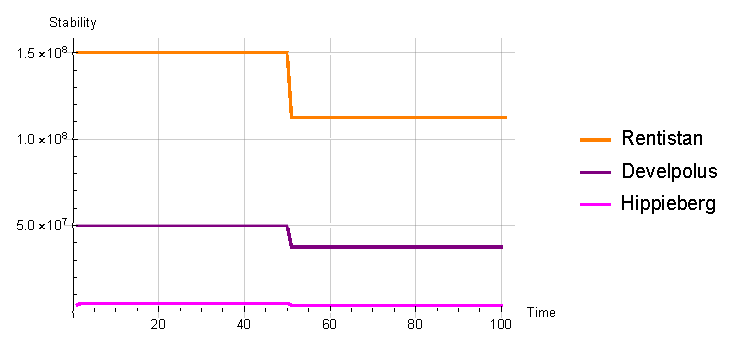
\includegraphics
[width=0.45\textwidth]{R_Shock_3.eps}}
\subfigure{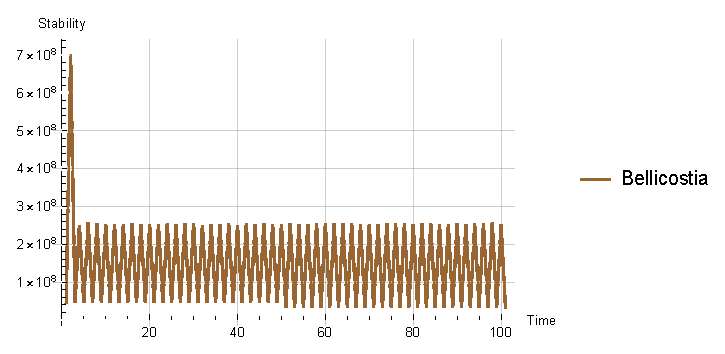
\includegraphics
[width=0.45\textwidth]{R_Shock_4.eps}} 
\subfigure{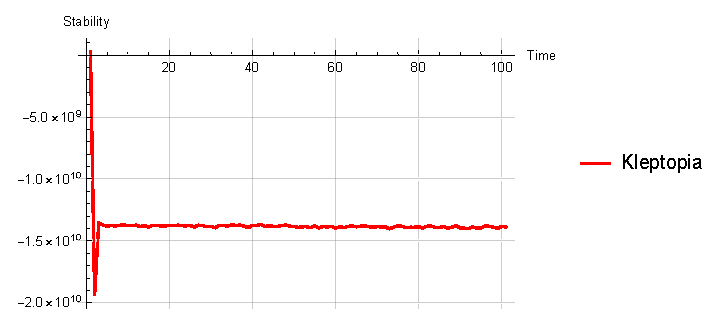
\includegraphics
[width=0.45\textwidth]{R_Shock_5.eps}}
\end{figure}

Figure 4 shows our countries reacting to a resource shock. Most of our countries show a substantial drop in stability after the hit to resources. Hippieberg, Bellicostia, and Kleptopia show the least amount of variation from the resource shock. A possible reason for this is that Hippieberg and Bellicostia already have a low amount of resources to begin with, so a further reduction in resources wouldn't have too much of an effect. Kleptopia is wealthy but autocratic, so it likely able to weather the shock without difficulty, though as before it at a negative level of stability.  

Freedonia and `Merika each see substantial drops in stability levels, but still maintain relatively high stability levels. The most interesting case is Rentistan, which suffers a high relative drop in stability. The fact that Rentistan seems the most vulnerable to a drop in resources makes sense given that the legitimacy of such regimes is often predicated upon their ability to provide for their citizens. When such a state is unable to provide the expected goods and services (or intimidate its citizens sufficiently) its stability will deteriorate. 

\subsubsection{Phi and Omega Shocks} 

\begin{figure}[htb]
\centering 
\caption{Phi Shock}
\subfigure{\includegraphics
[width=0.45\textwidth]{Phi_Shock_1.eps}} 
\subfigure{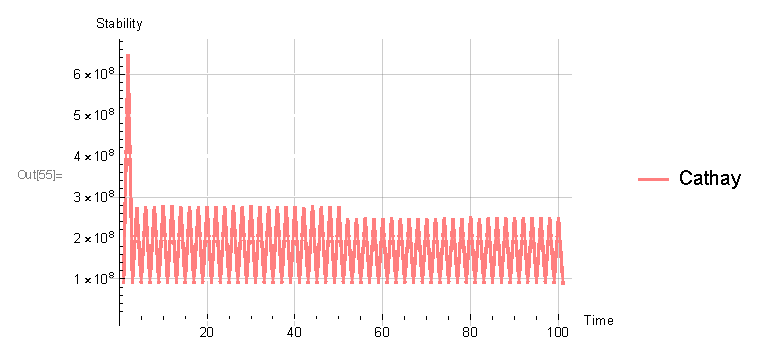
\includegraphics
[width=0.45\textwidth]{Phi_Shock_2.eps}} 
\subfigure{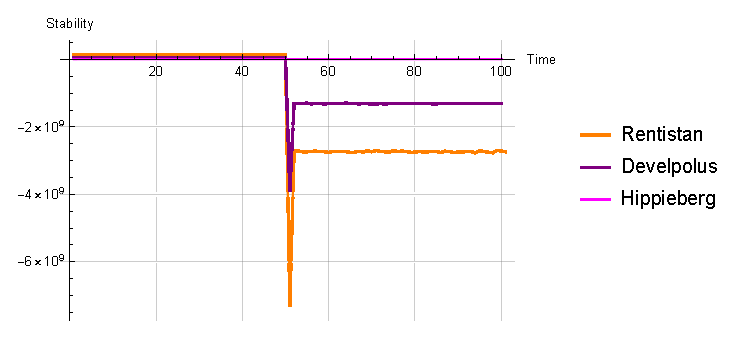
\includegraphics
[width=0.45\textwidth]{Phi_Shock_3.eps}} 
\subfigure{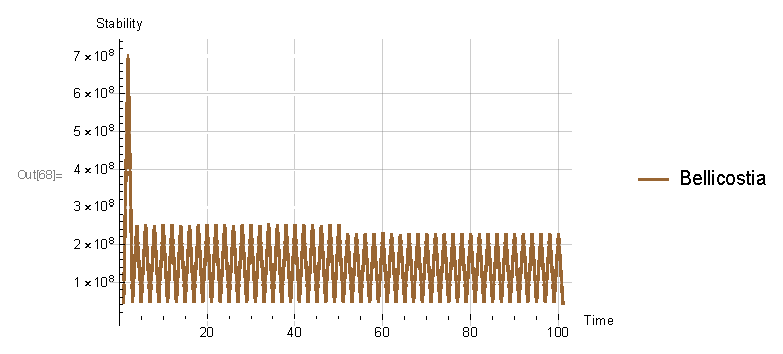
\includegraphics
[width=0.45\textwidth]{Phi_Shock_4.eps}}
\subfigure{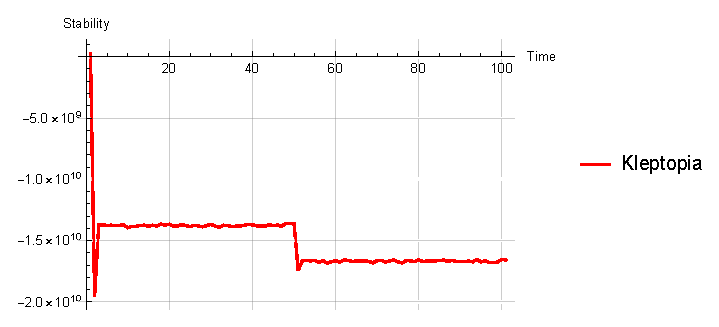
\includegraphics
[width=0.45\textwidth]{Phi_Shock_5.eps}}
\end{figure}

%Phi, government services 
Figures 5 and 6 depicts shocks to the anarchy parameters, $\Phi$ and $\Omega$, respectively. When there is a shock to minimum necessary government services, $\Phi$, it has quite the varied and counter-intuitive results across countries. Most curious, countries that place a preference on government services seem to suffer the least from the shock. Freedonia, `Merika, and Hippieberg show almost no change from the shock. Cathay and Bellicostia maintain their extreme oscillation, but after the shock each sees a decrease in the amplitude. Interestingly countries that take a more balanced or forceful stance; Rentistan, Develpolus, and Kleptopia, see extreme drops in stability. A possible reason why we get this result is that countries which take a balanced approach or favor suppression, provide a limited amount of government services to the public to begin with. Thus, if those limited services are further reduced, the effects of the shock are more aggressive than they would be for others.     


\begin{figure}
\centering
\caption{Omega Shock}
\subfigure{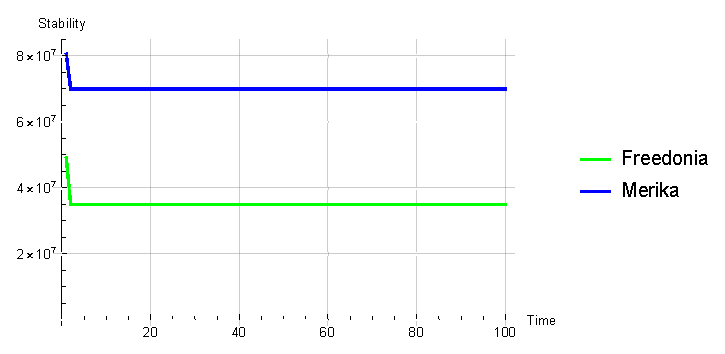
\includegraphics
[width=0.45\textwidth]{O_Shock_1.eps}} 
\subfigure{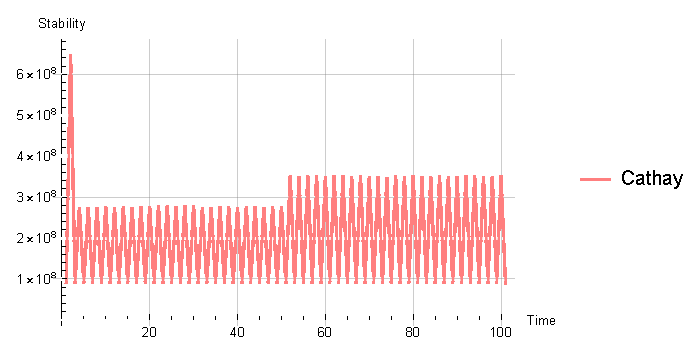
\includegraphics
[width=0.45\textwidth]{O_Shock_2.eps}} 
\subfigure{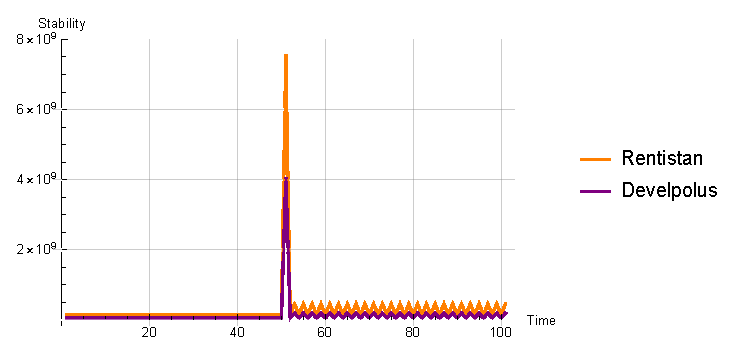
\includegraphics
[width=0.45\textwidth]{O_Shock_3.eps}} 
\subfigure{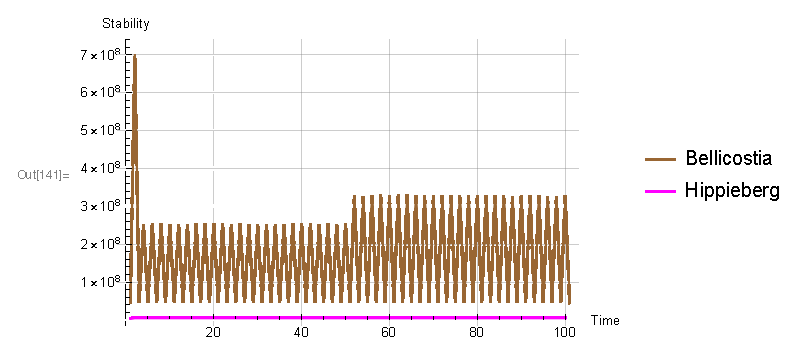
\includegraphics
[width=0.45\textwidth]{O_Shock_4.eps}}
\subfigure{\includegraphics
[width=0.45\textwidth]{O_Shock_5.eps}}
\end{figure}

The effects of a shock to security fixed costs, $\Omega$, has similar results as the shock to government services but differs in several interesting way. As with the Phi shock, Freedonia, `Merika, and Hippieberg show no substantial variation. Their structures are able to absorb the shock without much disruption to overall stability. Kleptopia is also able to weather the shock without fluctuating. Cathay and Bellicostia here have the opposite reaction as in the $\Phi$ shock, their amplitude increasing after the shock. The most interesting response is from Rentistan and Develpolus. The shock initially results in a massive spike in stability but then falls backdown into an oscillating pattern like Cathay and Bellicostia. %This is most likely a structural quirk than anything of note.   

%Why did I get this crazy result? 

\subsubsection{Environment Shock}

\begin{figure}
\centering
\caption{Environment Shock}
\subfigure{\includegraphics
[width=0.45\textwidth]{E_Shock_1.eps}} 
\subfigure{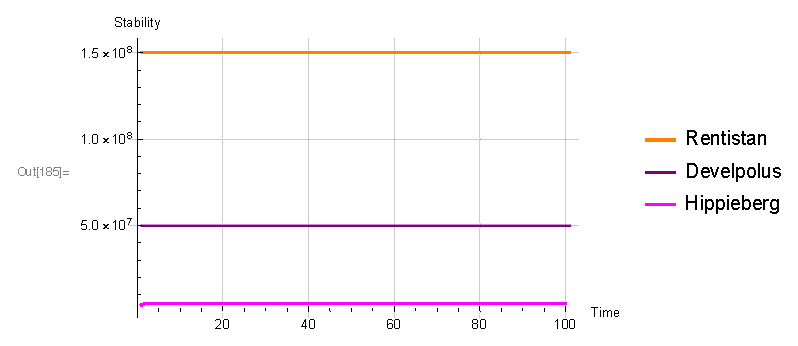
\includegraphics
[width=0.45\textwidth]{E_Shock_2.eps}} 
\subfigure{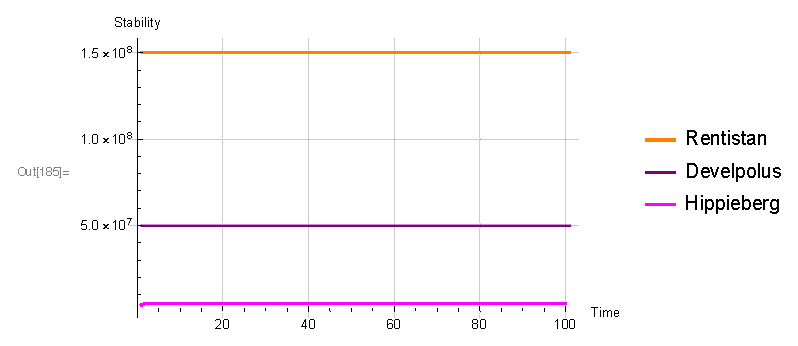
\includegraphics
[width=0.45\textwidth]{E_Shock_3.eps}} 
\subfigure{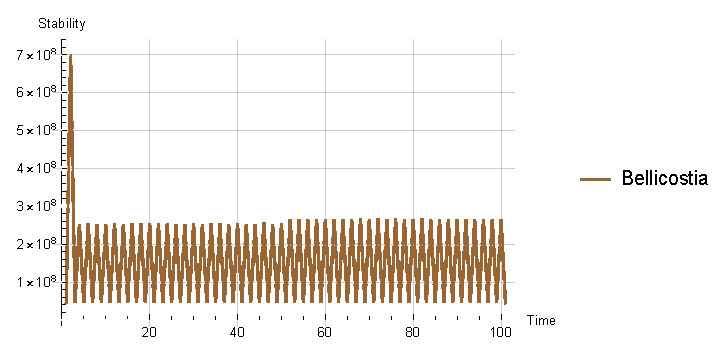
\includegraphics
[width=0.45\textwidth]{E_Shock_4.eps}}
\subfigure{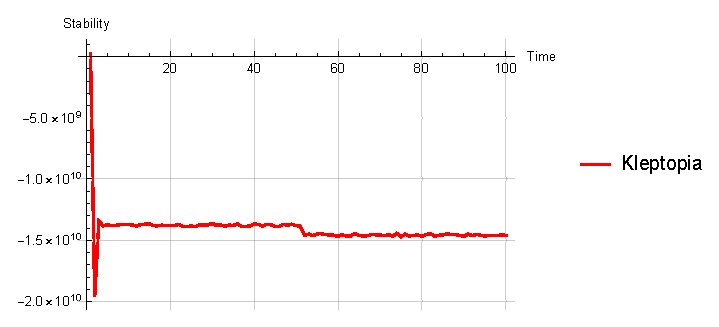
\includegraphics
[width=0.45\textwidth]{E_Shock_5.eps}}
\end{figure}


Figure 7 shows a shock to the citizen's environment/quality of life, $E$. Of all the shocks, a change in the average citizen's environment seems to have the least dramatic effect. Freedonia, `Merika, Rentisan, Develpolus, and Hippieberg show no visible change after the shock. Cathay and Bellicostia see a minor increase in amplitude, but one that is smaller than in other shocks. Kleptopia has strongest reaction, seeing a substantial drop in it's already negative stability. A possible reason why we see this minimal change with respect to an environmental shock is that a change in average citizen environmental wellbeing does not happen in isolation. Often it's precipitated by some other shock throughout the country, such as a resource shock, and the two compound one another. 


%should we do joint shocks?

\subsubsection{Enforcement Shock}

\begin{figure}
\centering
\caption{Enforcement Shock}
\subfigure{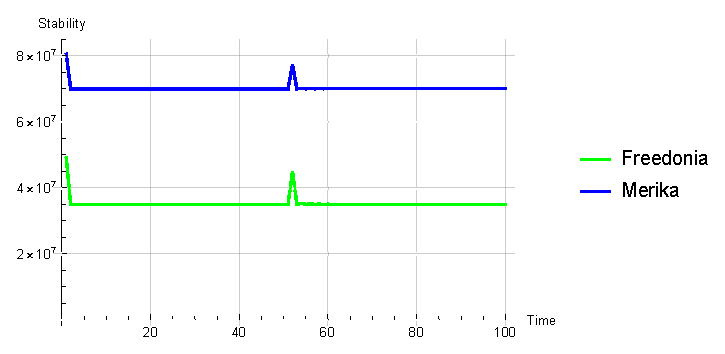
\includegraphics
[width=0.45\textwidth]{Es_Shock_1.eps}} 
\subfigure{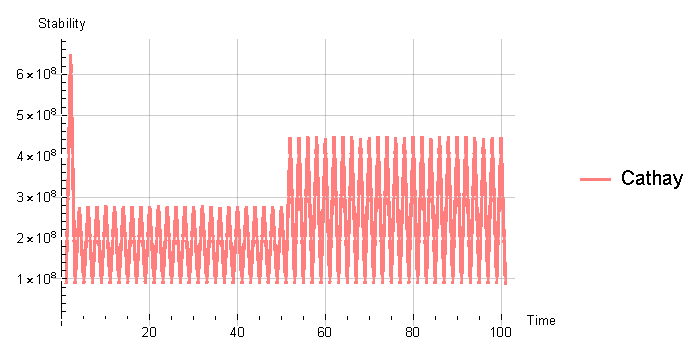
\includegraphics
[width=0.45\textwidth]{Es_Shock_2.eps}} 
\subfigure{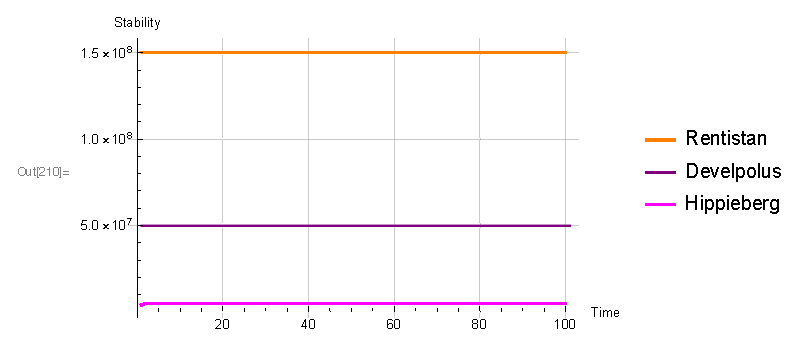
\includegraphics
[width=0.45\textwidth]{Es_Shock_3.eps}} 
\subfigure{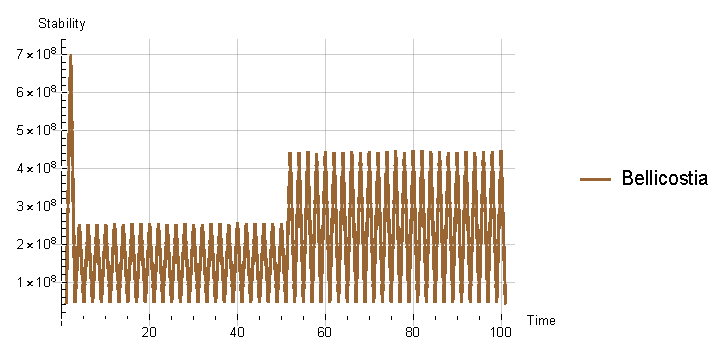
\includegraphics
[width=0.45\textwidth]{Es_Shock_4.eps}}
\subfigure{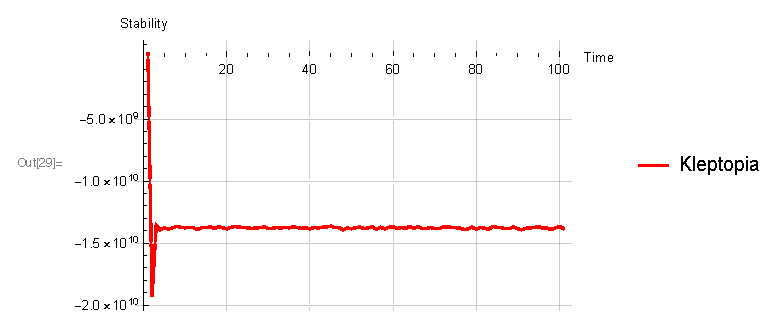
\includegraphics
[width=0.45\textwidth]{Es_Shock_5.eps}}
\end{figure}

Figure 8 shows a shock to policing effectiveness, $\sigma$. Bucking the results from the other simulations, here the most interesting result comes from Freedonia and `Merika. The initial enforcement shock causes a spike in stability for Freedonia and `Merika but then drops into a oscillating pattern that dampens back to pre-shock levels. Rentistan, Develpolus, Hippieberg, and Kleptopia show no change from the enforcement shock. Whereas, Cathay and Bellicostia see a substantial increase in the amplitude of their stability oscillations after the shock.  

%Simulation Summary 

While these simulations represent only a small handful of the infinite combinations possible, they are still highly informative as to the parameter relationships governing a country's stability. Overall, it seems that the most important factor affecting stability is government resources. Throughout the simulations, countries with the most resources displayed the most consistency in their stability. However, how one allocates those resources is the critical detail. Kleptoia, which has just as many resources as Freedonia and `Merika, was never able to achieve a positive level of stability. It would seem that a country cannot simply beat people into submission, they must provide some benefit to the populace as well. 

Another interesting result is extreme oscillation of Cathay and Bellicostia. Each was surprisingly robust to all the shocks, even though neither was able to reach a steady level of stability. In fact, averaging across time, Cathay and Bellicostia were the most stable states. However, the period to period change in stability, was also the greatest with the two. So in a short-run perspective these two would seem very unstable, but if one expands to see the whole picture we can see that they are stable in their instability. Situations like this might be why there are many seemingly politically unstable countries in the world, but large scale political revolution is relatively rare.   

\section{Conclusion}

Through this paper we believe we have formed a coherent theoretical narrative concerning the interactions of a government and its citizenry. Our simulations have shown that it is not only the resources of a state that matters in maintaining stability, but how a state allocates resource between government services and security as dictated by its preferences that dictates overall stability. Additionally we have shown that a state can be stable in its instability, oscillating dramatically between periods but maintaining a consistent pattern. Generally it would appear that there are sets of parameter values that form loose Nash equilibriums of stability, with some equilibriums appearing to be more robust to shocks than others.  

A short coming of this paper is that the model only applies to cases of internal strife and does not take into account the role of outside agitators. Additionally, this model presents a homogenous state, but could easily be expanded upon to a state where there is factionalization. However, it must be stated that this is a preliminary model with significant room for expansion in future research endeavors.

The importance of this work is that it establishes a framework for developing new measures of political stability, one that bridges the gap between the top and bottom viewpoints. Throughout this paper we have discussed the concept of aggregated dissent, $D$, but with only limited discussion of how to actually estimate this critical variable. Thankfully, advances and spread of social media technology make this paper more than a theoretical exercise. The companion piece to this paper will delve deeper into this.   

\end{spacing}


\pagebreak

\bibliographystyle{apalike}
\bibliography{Stability_Bibli}

\nocite{*}





\end{document}
